\documentclass[11pt, a4paper]{article}

\usepackage{graphicx}
\usepackage[a4paper,top=3cm,bottom=2cm,left=2cm,right=2cm,marginparwidth=1.75cm]{geometry}
\usepackage[english]{babel}
\usepackage[utf8x]{inputenc}
\usepackage{subfig}
\usepackage{float}
\usepackage{amsmath}
\usepackage{amssymb}
\usepackage{mhchem}
\usepackage{hyperref}
\usepackage{tikz}
\usepackage{cancel}
\usepackage{bm}

\graphicspath{ {./images} }
\newcommand*{\qed}{\hfill\ensuremath{\quad\square}}%
\newcommand*{\rad}{\ensuremath{\,\text{rad}}}
\newcommand*{\R}{\ensuremath{\mathbb{R}}}
\newcommand*{\C}{\ensuremath{\mathbb{C}}}
\renewcommand*{\Re}{\operatorname{Re}}
\renewcommand*{\Im}{\operatorname{Im}}
\renewcommand*{\epsilon}{\varepsilon}
\renewcommand*{\phi}{\varphi}
\renewcommand*{\d}{\text{d}}

\DeclareRobustCommand{\uvec}[1]{{%
  \ifcat\relax\noexpand#1%
    % it should be a Greek letter
    \bm{\hat{#1}}%
  \else
    \ifcsname uvec#1\endcsname
      \csname uvec#1\endcsname
    \else
      \bm{\hat{\mathbf{#1}}}%
     \fi
   \fi
}}

\makeatletter
\renewcommand*\env@matrix[1][*\c@MaxMatrixCols c]{%
  \hskip -\arraycolsep
  \let\@ifnextchar\new@ifnextchar
  \array{#1}}
\makeatother

\newtheorem{theorem}{Theorem}
\numberwithin{equation}{section}
\numberwithin{figure}{section}

%------------------------------------------------
%Templates for images and figures
% \begin{figure}[h]
%   \centering
%   \subfloat[caption 1]{{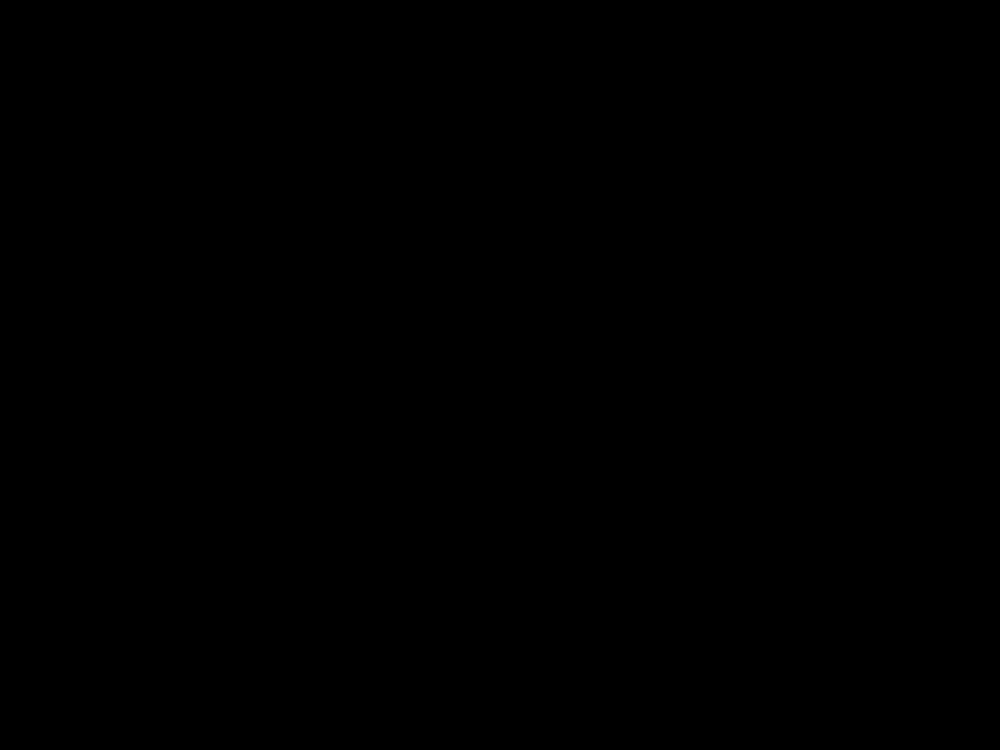
\includegraphics[width=30mm]{images/placeholder.png}}}%
%   \qquad
%   \subfloat[caption 2]{{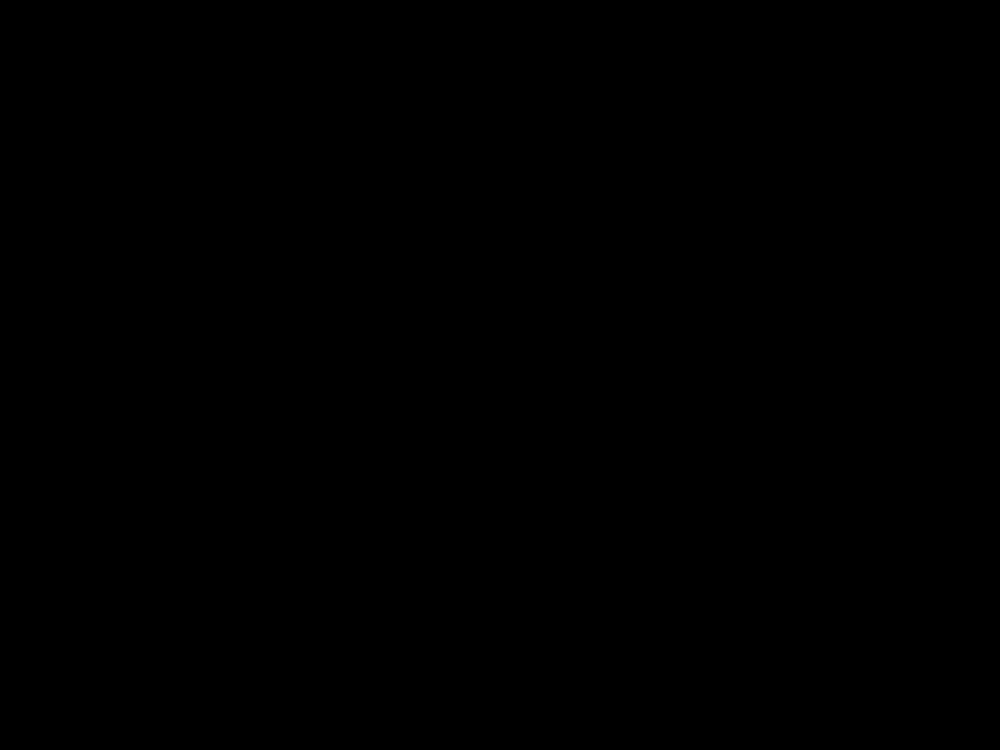
\includegraphics[width=30mm]{images/placeholder.png}}}%
%   \caption{Description}
% \end{figure}

% \begin{figure}[h]
%   \centerline{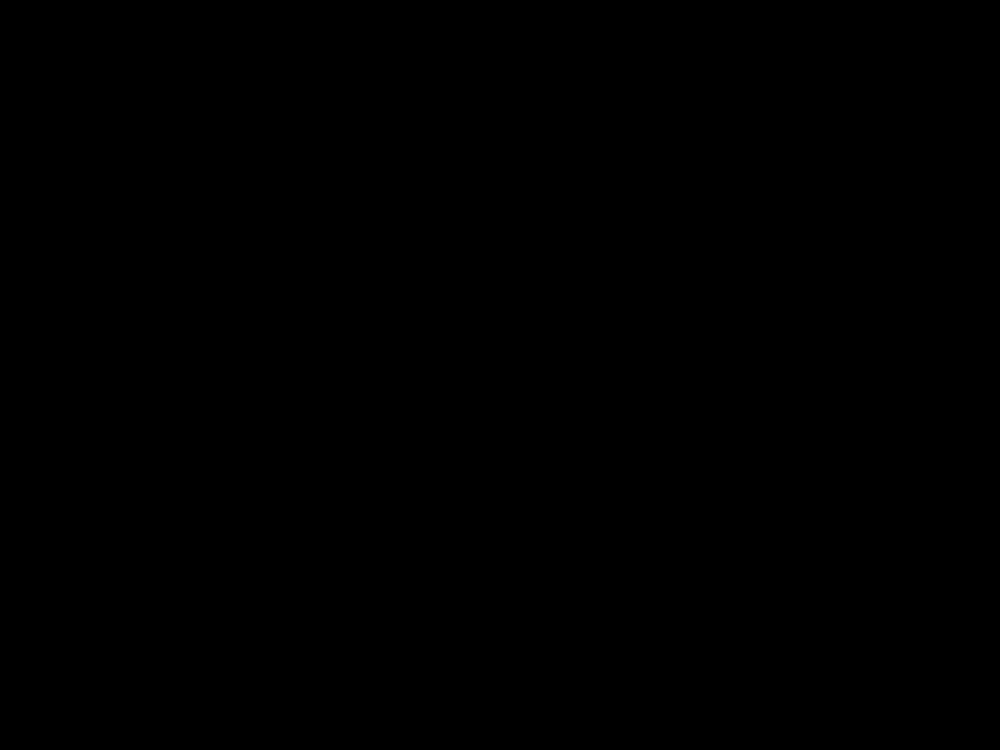
\includegraphics[width=50mm]{images/placeholder.png}}
%   \caption{Description}
% \end{figure}

%Template for a simple table 
%\begin{table}[h]
%   \caption{Description} %title of the table
%   \centering % centering table
%   \begin{tabular}{l rr} % creating three columns
%     \hline\hline %inserting double-line
%     & & \\ [0.5ex] % Insert half line vertical spacing
%     \hline % inserts single-line
%     & & \\ 
%     & & \\
%     & & \\
%     & & \\
%   \hline % inserts single-line
%   \end{tabular}
%   \label{tab:hresult}
% \end{table}
%-----------------------------------------------

\begin{document}
\setcounter{section}{1}

\section{Reliability}


\subsection{Level 1: Probability analysis}
Modelling up untill now has generally be done deterministically. This means some amount of neccesary variables are assumed, found in a table or found empirically. Then a worst case scenario is modeled to find some exact value. This is however not a very realistic approach as worst case scenario's never occur more then in $5\%$ of cases at the very most. It is instead sometimes usefull to convert our deterministic model to a probabilistic one. In this case we often model using a normal distribution (sometimes also called a Bell curve or Gaussian distribution.)\\
For our case study we will be looking at a part\footnote{use your imagination for which part this is.} which has a variable coefficient of friction. The models 2 types of models for this are given in the figure below.
\begin{figure}[h]
  \centering
  \subfloat[Uniform distribution]{{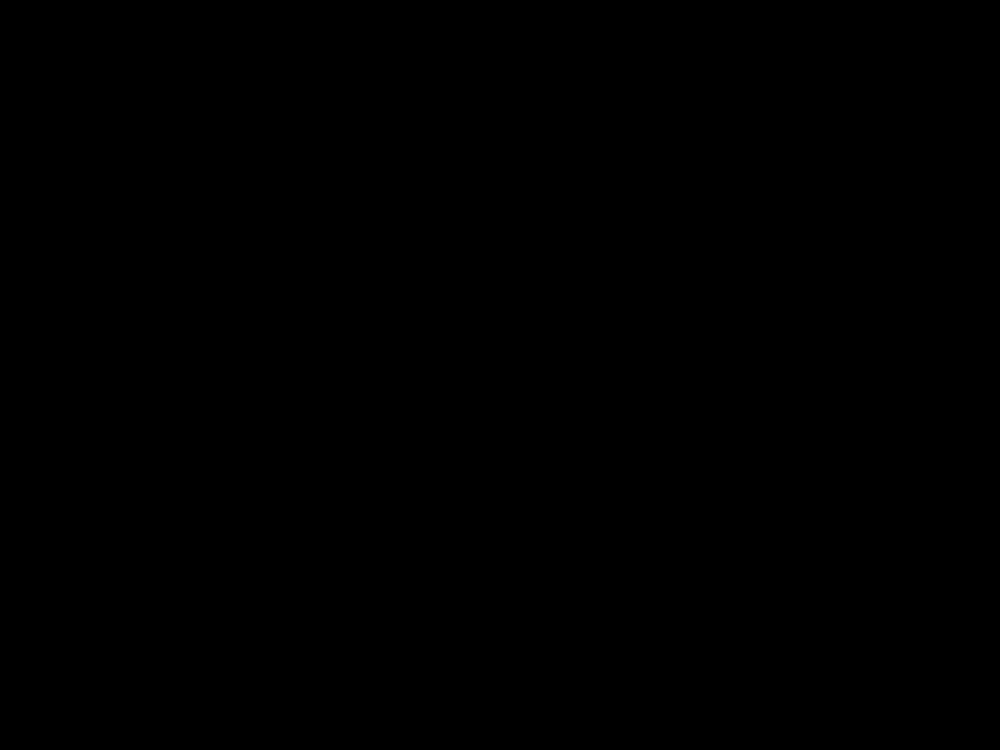
\includegraphics[width=60mm]{images/placeholder.png}}}%
  \qquad
  \subfloat[Gaussian distribution]{{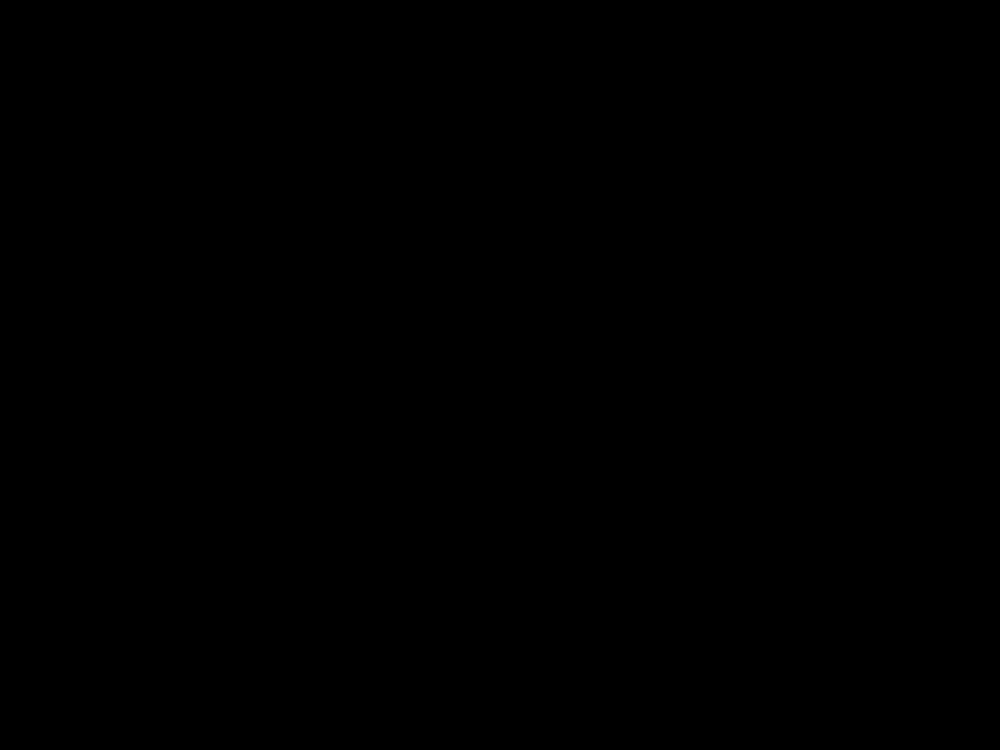
\includegraphics[width=60mm]{images/placeholder.png}}}%
  \caption{The distribution of possible coefficients of friction of the bearing modeled in 2 different types of distribution}
\end{figure}
We want to find the minimal coefficient of friction of with a maximum of $5\%$ chance to exceed this value. On a uniform distribution we can easily see that this value is $0.16$, howver this is very unrealistic. Normally we expect the amount of samples closer the mean value $\mu$ to be larger then the amount of samples closer to some amount of standard deviations away from the mean value. When modeling using a normal distribution we know the following values:
\begin{equation*}
  \mu = 0.25 \quad \sigma = \frac{0.1}{3} \quad f(t) = \frac{1}{\sigma\sqrt{2\pi}} \cdot \exp\left( \frac{(-t-\mu)^2}{2\sigma^2} \right)
\end{equation*}
We also know that:
\begin{gather*}
  x_{min} = 0.15\\
  x_{max} = 0.35
\end{gather*}
We want to find the point $t_1$ where the area under the bell curve is less then $5\%$:
\begin{equation*}
  F(t_1) = \int_{-\infty}^{t_1} f(t)\,\d t
\end{equation*}
When solving this we find that $t_1 = 0.1953$. Having to constantly eveluate the integral at different values to find probabilities is quiet cumbersome. Instead we can apply a standard model of a Gaussian distribution with mean value $\mu = 0$ and standard deviation $\sigma=1$ and tabulate the results. We call these $z$-tables. We can find some value for $z$ in the table and then convert that to apply it to our situation with different $\mu$ and $\sigma$. An example of a $z$-table is given below. The equations that apply to a $z$-table are as follows:
\begin{equation*}
  f(z) = \frac{1}{\sqrt{2\pi}}\exp\left( \frac{-z^2}{2} \right)
\end{equation*}
Where:
\begin{gather*}
  x_{min} = -3\\
  x_{max} = 3
\end{gather*}
\begin{table}[h]
  \caption{A $z$-table. This can be expanded using the equations listed above.} %title of the table
  \centering % centering table
  \begin{tabular}{l rrrrrr} % creating three columns
  \hline
   $F(z)$ & $0.5$ & $0.75$ & $0.80$ & $0.90$ & $0.925$ & $0.95$ \\ 
    $z$   & $0.0$ & $0.67$ & $0.84$ & $1.03$ & $1.44$  & $1.64$ \\
  \hline % inserts single-line
  \end{tabular}
\end{table}
In our case we for finding the coefficient of friction we had:
\begin{equation*}
  \mu = 0.5 \quad \sigma = \frac{0.1}{3}
\end{equation*}
For a probability of $5\%$ we find that $z_1 = 1.64$. Converting this back to our value $t_1$ we want to find is done with the following equation:
\begin{equation}
  t' = \mu - z_1\sigma
\end{equation}
Which in our case evaluates back to $0.1953$ which is the same as what we found using the intgral. Thus we can conclude that the coefficient of friction will be higher then $0.1953$ in $95\%$ of the cases.


\subsection{Level 2: Variability analysis}
Quality is how well a product conforms to the requirements. Reliability is how well the performance of said product can be predicted.
Consider a brake system on a bike. requirements of the braking system is deceleration. It should be predictable, repeatable and reliable. The parameters which influence friction are the frictional force and the coefficient of friction. We assume the wrap angle of the bowden cables is $\pi \rad$. Our C.o.F. is given as $\mu = 0.15\pm,0.05$. We can now use the Capstan equation to find that:
\begin{align}
  \frac{T_1}{T_2} &= \exp(\mu \alpha)\,,\,T_1\geq T_2\\
                  &= 1 - \exp(-\mu\alpha)\notag\\
                  &= 0.37\pm0.1\notag
\end{align}
The percentage of Tensile force lost due to firction is $37\%$ with $\pm27\%$ variation from the mean value. When considering the brake handle as a Mechanical amplifier we find that
\begin{equation}
  \begin{cases}
    F_2 = F_1\frac{L_1}{L_2}\\
    F_3 = F_2\eta\,,\,\eta = 1 - \frac{T_1 - T_2}{T_1}\\
    F_{brake} = \mu F_3
  \end{cases}
\end{equation}
When subsituting those equations into eachother we find an expression for brake force which takes the following forms:
\begin{equation}
  F_{brake} = axy
\end{equation}
Where $a$ is a real constant and $x$ and $y$ are the independent parameters which influence the brake force. Using some mathematics for uncorrelated values we find that:
\begin{equation}
  \mu_{axy} = a\mu_x\mu_y\\
  \sigma_{axy} = a\sigma_{xy}
\end{equation}
Where $\mu$ is the mean and $\sigma$ the standard deviation. When optimizing this we try to minimize the coefficient of variation which is given as:
\begin{equation}
  c_v = \frac{\sigma}{\mu}
\end{equation}
Some rules for mathematics of uncorrelated variables:
\begin{itemize}
  \item[] $\sigma_{x\pm y} = \sqrt{\sigma_x^2 + \sigma_y^2}$
  \item[] $\sigma_{ax + b} = \sqrt{a^2\sigma_x^2} = a\sigma_x$
  \item[] $\sigma_{xy} = \sqrt{\sigma_x^2\sigma_y^2 + \sigma_x^2\mu_y^2 + \sigma_y^2\mu_x^2}$
\end{itemize}


\subsection{Level 3: Optimization techniques}
For optimization, as stated before, we try to minimize the coefficient of variation $c_v$. A common approach for this is a top-down approach. The is usually coupled with a Foult Tree Analysis (FTA). It is a way of graphically representing possible system failures. For this approach the general outline is given as:
\begin{enumerate}
  \item Identify possible system failures
  \item Construct a fault tree with logic operators
  \item Establish the system Reliability $R(t)$
  \item identify critical components/paths
\end{enumerate} 

\subsubsection{Components connected in series}
For components in series a failure in 1 component causes failure of the whole system. Thus we find the total reliability by multiplying them all together:
\begin{equation}
  R_{system}(t) = \prod_{j=1}^n R_j(t)
\end{equation}
Typical examples of systems in series are LRC-circuits (used for various signal filters) and drive trains.


\subsubsection{Components connected in parallel}
Reliability for parallel systems increases with more components rather then decreases. This is called parallel redundancy. The total reliability of a parallel system is given as:
\begin{equation}
  R_{system}(t) = 1 - \prod_{j=1}^n (1 - R_j(t))
\end{equation}
Typical examples of parallel systems are fans in a computer case.


\subsubsection{Failure mode and Effective Anlysis (FMEA) and Root Cause Analysis (RCA)}
For complete failure analysis FMEA can be usefull to identify critical components, rate the probability of failure and the impact of failure for a given system. It is usually performed by a multi-disciplinary team and can be used as the basis for the failure tree.
RCA is used for finding the Root cause of failures. The failure itself is the function loss or sometimes called failure mode. The root cause of the failure is the failure mechanism such as corrosion, exceeding of UTS, etc. Failure mechanisms are of vital importance for determining which corrective action should be takes.

\end{document}